\chapter{Demo cases}
\section{2D cavity flow at $\text{Kn}=0.075$}
\label{sec_cavity}
This demonstrational case is provided in the \verb|demos| subdirectory of the dugksFoam source code package.
This case is a popular benchmark problem for validating numerical method for micro or rarefied gas flows.
It has been studied in Ref.~\cite{zhulh15} using this solver,
where you can find the detailed description of this problem.
We only mention some setting that need special attention for a new user.
The mesh file and setting have already been prepared in the case directory.
So you can run the dugksFoam directly.

The flow configuration is illustrated in Fig.~\ref{ldc}.
The walls are diffusive boundaries.
For such a simple geometry, you can use the \verb|blockMesh| shipped with the OpenFOAM to generate the structured mesh.
Refer to the cavity flow tenurial case in the \emph{OpenFOAM User's Guide} for the detailed usage of \verb|blockMesh|.
The initial temperautre filed is uniform 273K, and the wall temperature is also 273K.
In this case, the Knudsen number Kn is 0.075 based on the initial density filed and the cavity width $L$.
So the mean free path is 0.075m.
The initial density field input in the \verb|0/rho| file should be calculated from the mean free path provided the argon gas properties.
Refer to ~\cite{zhulh15} for the related formulations.
We also provide a simple Python script named \verb|para.py| in the case's directory to compute the related parameters.
You can run it by \verb|python para.py|.


The discrete velocities used are $28\times28$ half-range Gauss-Hermite quadrature points.
The files \verb|constant/Xis| and \verb|constant/weights| can be generated by
\begin{verbatim}
    setDV.py GH 337.196399395 28
\end{verbatim}
where 28 is the number of discrete velocity in each direction, and 337.196399395 stands for the most probable speed of argon gas molecular at $T=273$K.
Refer to Sec.~\ref{sec_dv} for more details about settings of discrete velocities.

Fig.~\ref{ldc_UT} show some of the results of this case.
You can also compare the results with those in \cite{zhulh15} in detail.

\begin{figure}
  \centering
  % Requires \usepackage{graphicx}
  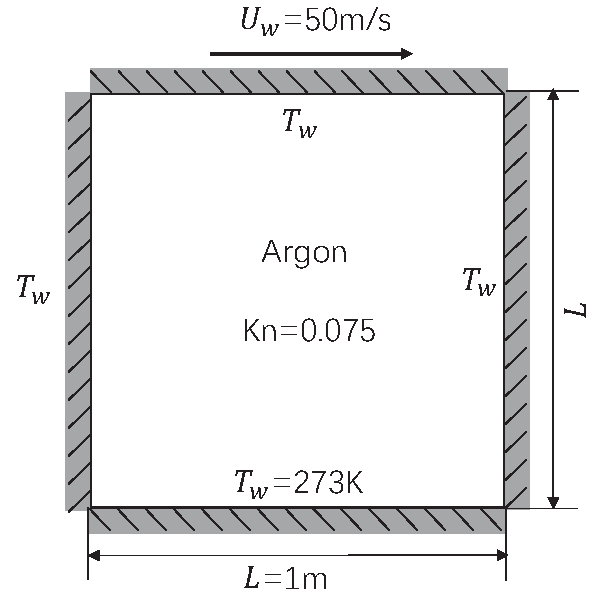
\includegraphics[width=0.4\textwidth]{img/ldc.pdf}
  \caption{Lid-driven cavity flow}\label{ldc}
\end{figure}

\begin{figure}[htbp]
\centering
\subfloat[]{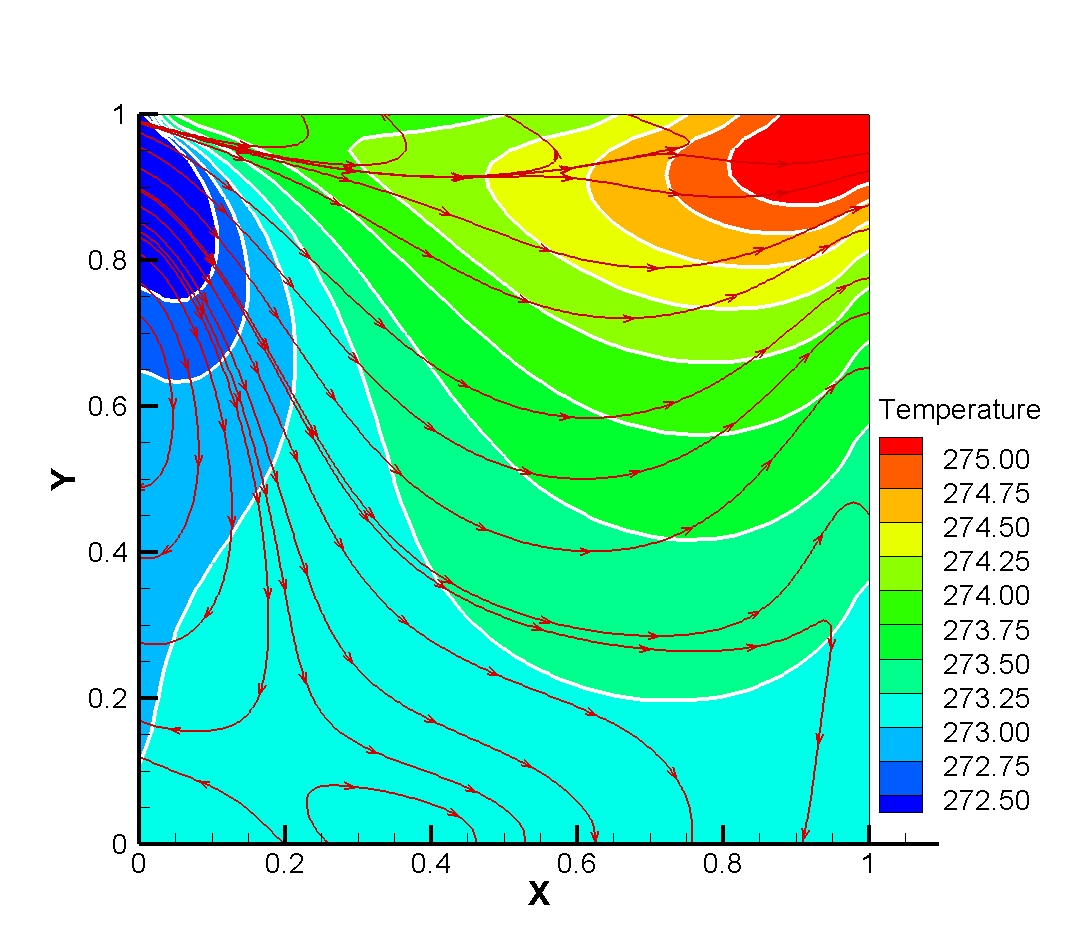
\includegraphics[width=0.48\textwidth]{img/temperature.png}} ~
\subfloat[]{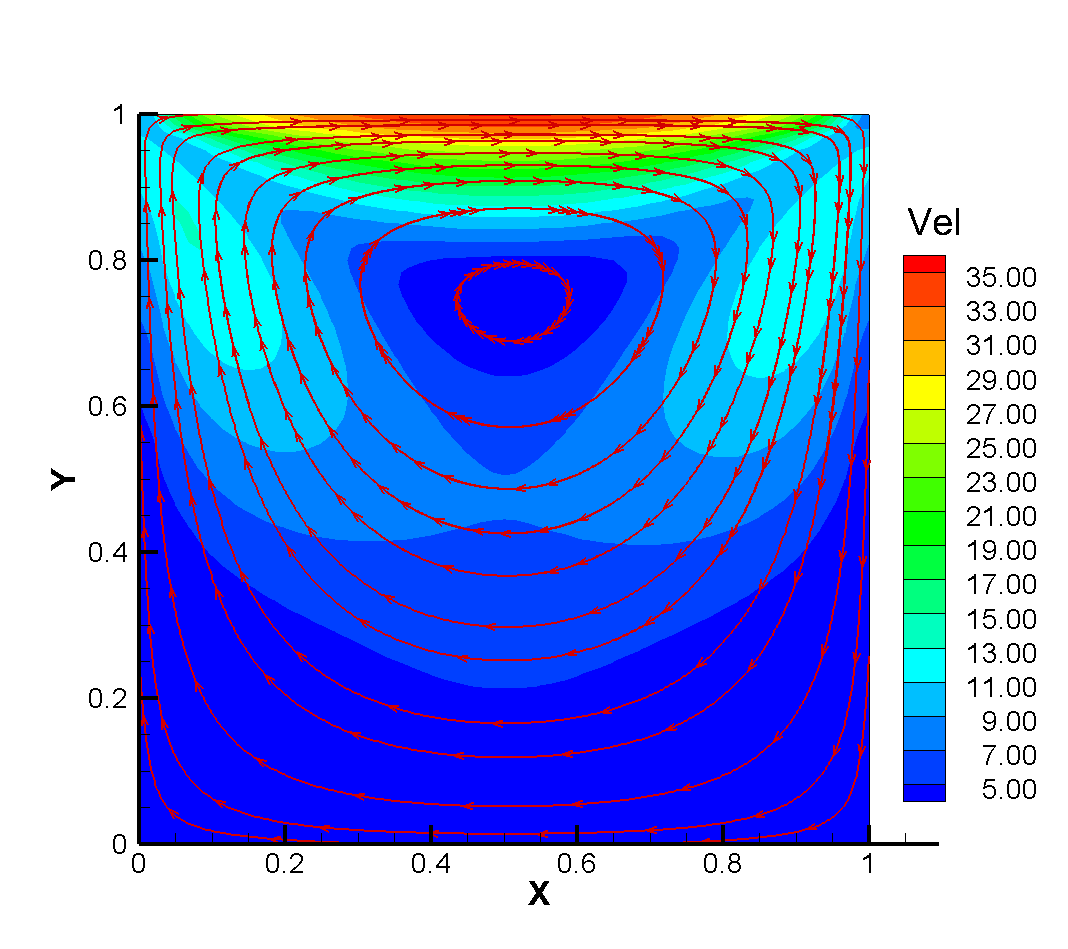
\includegraphics[width=0.48\textwidth]{img/U.png}}
\caption{
Results of the cavity flow case. (a) Temperature contours and heat flux. (b) Velocity magnitude and streamlines.
}\label{ldc_UT}
\end{figure}

% Local Variables:
% TeX-master: "dugksFoam"
% mode: latex
% mode: flyspell
% End:
